



\begin{minipage}{0.65\textwidth}
\begin{figure}[ht]
    \centering
    \rotatebox{90}{\hspace{8mm}\scalebox{0.8}{$B_0=700\un{Гс}$ \hspace{16 mm} $B_0=300\un{Гс}$}}
    \hspace{1 mm} 
    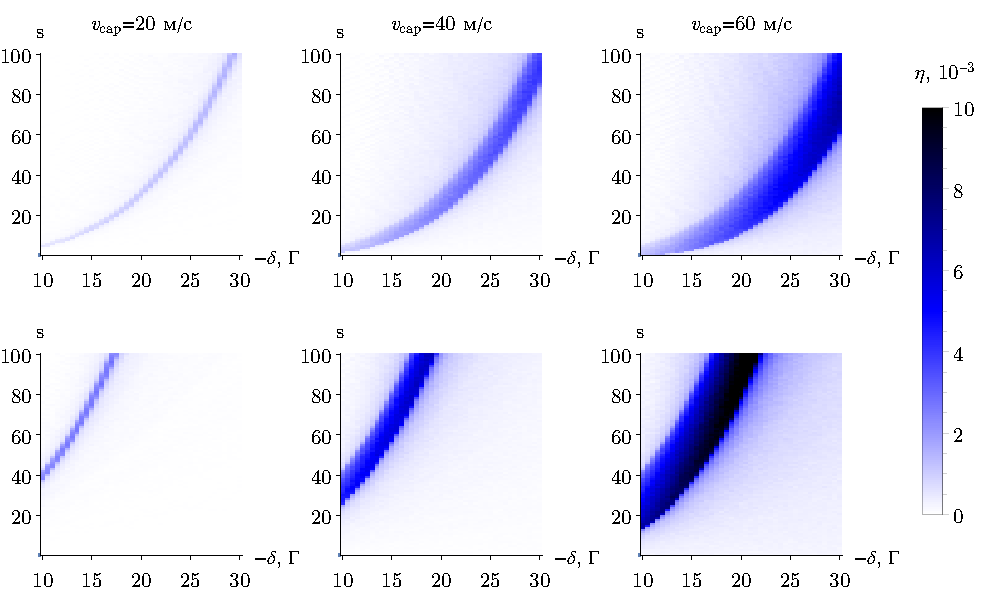
\includegraphics[width=0.94\textwidth]{../MOT/figs/etas_v4.pdf}
    \caption{Зависимость эффективности работы замедлителя $\eta$ от отстройки луча ЗЗ $\delta$, параметра насыщения $s$ для двух различных значений амплитуды магнитного поля в ЗЗ}
\end{figure}

\end{minipage}
\hfill
\begin{minipage}{0.31\textwidth}



Загрузка в МОЛ: $\ v < \sub{v}{cap}$

\phantom{42}

$\eta = \frac{\sub{\Phi}{load}}{\sub{\Phi}{sol}}$ -- эффективность ЗЗ

\phantom{42}

\begin{figure}[h]
    \centering
    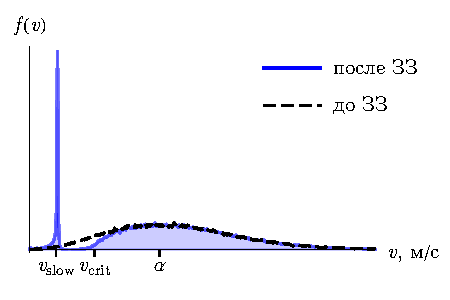
\includegraphics[scale=0.66]{../MOT/figs/vdist_v5.pdf}
    \caption{Преобразование распределения атомов по скоростям после ЗЗ}
    %\label{fig:}
\end{figure}


\end{minipage}